\chapter{GUI-Entwurf}
In diesem Kapitel werden die Komponenten der grafischen Benutzeroberfläche der Eventverwaltungssoftware sowie deren Zusammenspiel erläutert. Auch für die Entwicklung der Benutzeroberfläche wird auf Klassen und Interfaces aus den swe-utils zurückgegriffen, welche im nachfolgenden Abschnitt genauer erläutert werden. Auch die Komponenten der Benutzeroberfläche wurden in Pakete eingeteilt, welche sich an der Struktur der im Entwurfsklassendiagramm modellierten Pakete \enquote{model} orientieren. Deren jeweilige Funktion wird im Anschluss an die Komponenten aus den swe-utils erklärt.

\begin{figure}[ht!]
    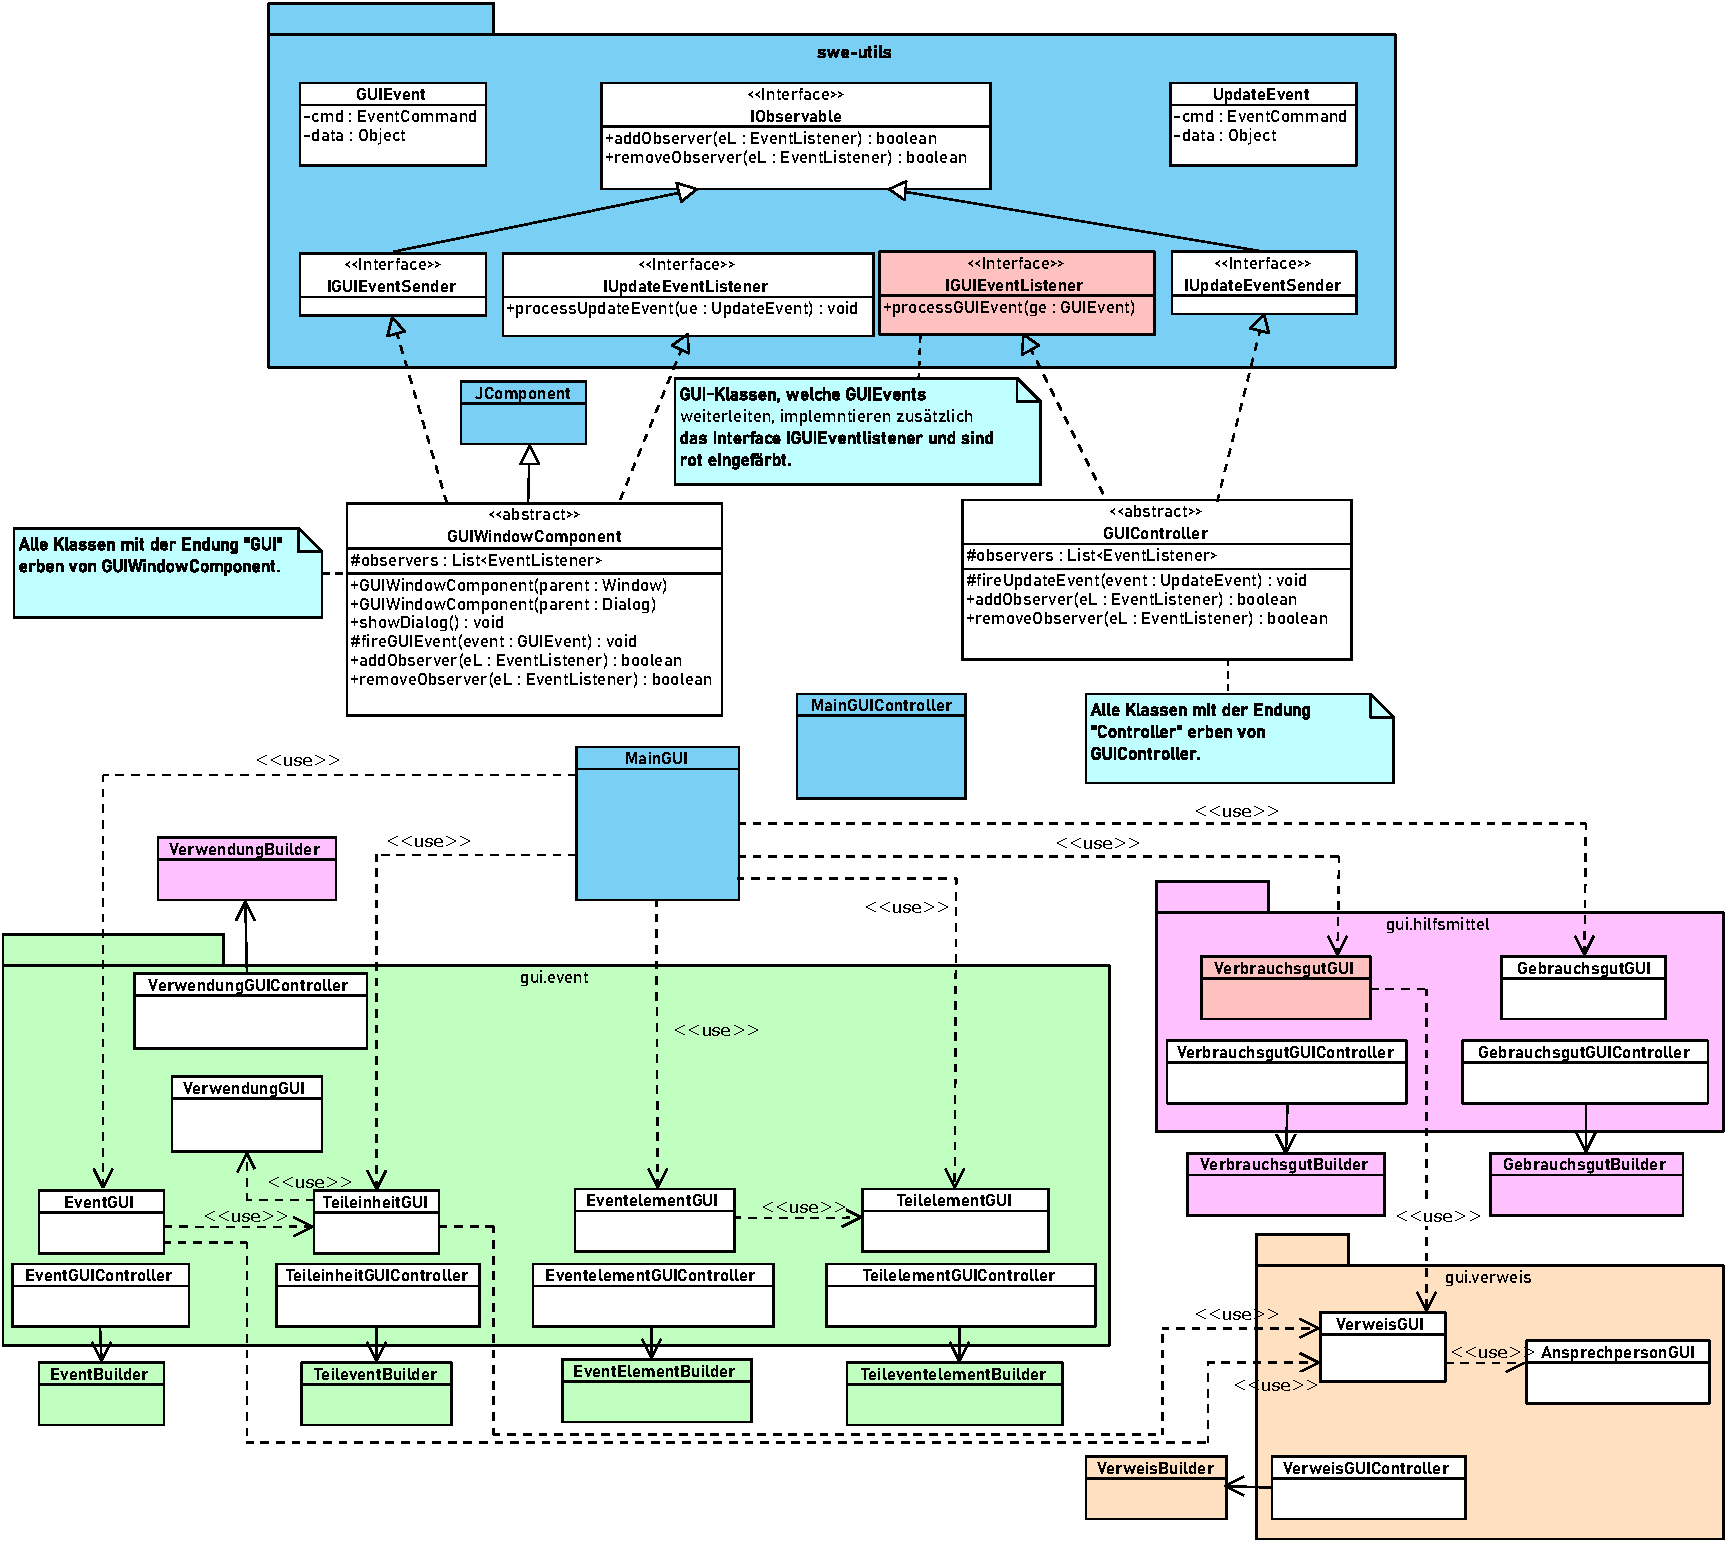
\includegraphics[width=0.98\columnwidth]{Bilder/ekd_GUI.pdf}
    \caption{Entwurfsklassendiagramm der GUI}
\end{figure}

\section{swe-utils}
Als Grundlage des GUI-Entwurfes werden zur Umsetzung des Observerpatterns Interfaces aus den swe-utils verwendet. Für von einem View ausgehende Signale an Controller werden GUIEvents verwendet, für von einem Controller an den View gehende Signale hingegen werden UpdateEvents verwendet. Diese beiden Klassen haben jeweils einen EventCommand und Nutzdaten. Diese Daten sind dabei allgemein gehalten und der EventCommand ist ebenfalls lediglich eine Oberklasse, die von den einzelnen Sender-Klassen mit jeweils einem Commands-Enum erweitert wird.

Die Interfaces \enquote{IGUIEventSender} und \enquote{IGUIEventListener} bilden die Kommunikation von View zu Controller ab. Alle Views erben von \enquote{GUIWindowComponent}, welches \enquote{IGUIEventsender} implementiert und sendet damit GUIEvents an die GUIController, welche \enquote{IGUIEventListener} implementieren.

Entsprechend andersherum ist die Kommunikation von Controller zu View modelliert: Der \enquote{GUIController} implementiert das Interface \enquote{IUpdateEventSender} und sendet damit UpdateEvents an den View, welcher \enquote{IUpdateEventListener} implementiert.

Die beiden Interfaces \enquote{IGUIEventSender} und \enquote{IUpdateEventSender} erben von \enquote{IObservable}, denn sie bilden beide jeweils das Observable im Observerpattern ab. Dafür müssen Methoden zum Hinzufügen und Entfernen von Observern implementiert werden.

Die Klassen \enquote{GUIWindowComponent} und \enquote{GUIController} sind jeweils abstrakte Klassen, von denen die konkreten Views und Controller erben. Sie stellen eine Basis gemeinsamer Funktionalität dar, die das umsetzen des Observerpatterns ermöglicht. Die Klasse \enquote{GUIWindowComponent} erbt dafür von \enquote{JComponent}, welche es ermöglicht, die Views flexibel in einem \enquote{JFrame}, \enquote{JDialog} oder als Komponente in einem \enquote{JPanel} zu verwenden.

\section{Struktur der GUI}
Den Einstiegspunkt der Benutzeroberfläche bildet die \enquote{MainGUI}, welche für jede der Grundfunktionen der Software, wie beispielsweise die Verwaltung von Events, Mitarbeitern oder Hilfsmitteln einen eigenen Tab enthält, welcher wiederum eine tabellarische Übersicht über die vorhandenen Elemente enthält sowie die Möglichkeit, Unter-UIs aufzurufen, um die Elemente detaillierter zu betrachten und zu bearbeiten. 

Das gesamte GUI-Paket besteht aus drei Unterpaketen: Das Paket \enquote{gui.event} enthält alle UI-Komponenten zur Erstellung von Events. Die EventGUI kann hierbei die TeileinheitGUI sowie die VerweisGUI instanziieren, da jedem Event Verweise sowie Teileinheiten hinzugefügt werden können. Die TeileinheitGUI kann ebenfalls die VerweisGUI sowie die VerwendungGUI instanziieren, da für Aktionen auch Hilfsmittel gebucht werden können, was mittels einer Verwendung geschieht.

Das Paket \enquote{gui.event} enthält auch die GUI-Komponenten zur Erstellung von Eventelementen und Teilelementen. Da einem Eventelement auch Teilelemente hinzugefügt werden können, kann die EventelementGUI die TeilelementGUI instanziieren. Das Paket \enquote{gui.verweis} enthält alle notwendigen Komponenten zur Erstellung von Verweisen, hierzu zählt auch das Anlegen von Ansprechpersonen zu einem Verweis, was in einem separaten UI geschieht. 

Die VerweisGUI wird neben den oben beschriebenen GUIs auch von der VerbrauchsgutGUI zum Anlegen von Verbrauchsgütern instanziiert, da zu diesen stets ein Lieferant in Form eines Verweises hinterlegt wird. Diese GUI gehört ebenso wie die GebrauchsgutGUI zum Anlegen von Gebrauchsgütern zum Paket \enquote{gui.hilfsmittel}. Jede der eben beschrieben UIs wird auf Kundenwunsch durch ein eigenes Fenster realisiert.

\section{Kommunikation der GUI-Komponenten}
Da die gesamte Benutzeroberfläche nach dem Model-View-Controller-Pattern entwickelt wurde, existieren zu jeder dieser UIs drei Klassen: Eine Viewklasse, welche die anzuzeigenden UI-Elemente definiert und vom Benutzer ausgelöste Signale in Form von GUIEvents an die jeweilige Controllerklasse weitergibt, bzw. Steuersignale in Form von Update-Events von dieser empfängt. Bei diesen Viewklassen handelt es sich jeweils um die Klassen mit der Endung \enquote{GUI}. Zu jeder Viewklasse existiert außerdem eine Controllerklasse, welche die GUIEvents von den Viewklassen empfängt, verarbeitet und Steuersignale an die Viewklassen sendet. Die Kommunikation zwischen diesen beiden Klassen erfolgt lediglich mittels den eben genannten Events und realisiert damit das Observerpattern. Jeder Controller hält eine Referenz auf eine Builderklasse für die jeweilige Entität. Diese realisiert das Builderpattern und hält die durch den Benutzer eingegeben Daten bis dieser auf den Sichern-Knopf klickt. Dann wird mittels der Builderklasse das entsprechende Objekt gebaut und mit Hilfe der im Entwurfsklassendiagramm beschriebenen EntityFactory und des jeweiligen EntityManagers persistiert.

Eine Ausnahme bildet hier der MainGUIController, welcher als einziger keine Builderklasse referenziert, da die MainGUI keiner bestimmten Entität zugeordnet ist. Außerdem besitzt die AnsprechpersonGUI keinen eigenen Controller, da Ansprechpersonen lediglich bei Verweisen angelegt werden können. Aus diesem Grund wird die AnsprechpersonGUI durch den entsprechenden VerweisGUIController gesteuert. Ferner sind manche der Viewklassen rot eingefärbt, um zu kennzeichnen, dass diese zusätzlich das Interface \enquote{IGUIEventListener} implementieren, da sie GUIEvents untergeordneter GUIs an ihren Controller weiterleiten.
